\documentclass[paper=letter,11pt]{scrartcl}

\KOMAoptions{headinclude=true, footinclude=false}
\KOMAoptions{DIV=14, BCOR=5mm}
\KOMAoptions{numbers=noendperiod}
\KOMAoptions{parskip=half}
\addtokomafont{disposition}{\rmfamily}
\addtokomafont{part}{\LARGE}
\addtokomafont{descriptionlabel}{\rmfamily}
%\setkomafont{pageheadfoot}{\normalsize\sffamily}
\setkomafont{pagehead}{\normalsize\rmfamily}
%\setkomafont{publishers}{\normalsize\rmfamily}
\setkomafont{caption}{\normalfont\small}
\setcapindent{0pt}
\deffootnote[1em]{1em}{1em}{\textsuperscript{\thefootnotemark}\ }


\usepackage{amsmath}
\usepackage[varg]{txfonts}
\usepackage[T1]{fontenc}
\usepackage{graphicx}
\usepackage{xcolor}
\usepackage[american]{babel}
% hyperref is needed in many places, so include it here
\usepackage{hyperref}

\usepackage{xspace}
\usepackage{multirow}
\usepackage{float}


\usepackage{braket}
\usepackage{bbm}
\usepackage{relsize}
\usepackage{tcolorbox}

\def\ketY{\ensuremath{\ket {\Psi}}}
\def\iGeV{\ensuremath{\textrm{GeV}^{-1}}}
%\def\mp{\ensuremath{m_{\textrm{proton}}}}
\def\rp{\ensuremath{r_{\textrm{proton}}}}
\def\me{\ensuremath{m_{\textrm{electron}}}}
\def\aG{\ensuremath{\alpha_G}}
\def\rAtom{\ensuremath{r_{\textrm{atom}}}}
\def\rNucl{\ensuremath{r_{\textrm{nucleus}}}}
\def\GN{\ensuremath{\textrm{G}_\textrm{N}}}
\def\ketX{\ensuremath{\ket{\vec{x}}}}
\def\ve{\ensuremath{\vec{\epsilon}}}


\def\ABCDMatrix{\ensuremath{\begin{pmatrix} A &  B  \\ C  & D \end{pmatrix}}}
\def\xyprime{\ensuremath{\begin{pmatrix} x' \\ y' \end{pmatrix}}}
\def\xyprimeT{\ensuremath{\begin{pmatrix} x' &  y' \end{pmatrix}}}
\def\xy{\ensuremath{\begin{pmatrix} x \\ y \end{pmatrix}}}
\def\xyT{\ensuremath{\begin{pmatrix} x & y \end{pmatrix}}}

\def\IMatrix{\ensuremath{\begin{pmatrix} 0 &  1  \\ -1  & 0 \end{pmatrix}}}
\def\IBoostMatrix{\ensuremath{\begin{pmatrix} 0 &  1  \\ 1  & 0 \end{pmatrix}}}
\def\JThree{\ensuremath{\begin{pmatrix}    0 & -i & 0  \\ i & 0  & 0 \\ 0 & 0 & 0 \end{pmatrix}}} 
\def\JTwo{\ensuremath{\begin{bmatrix}    0 & 0 & -i  \\ 0 & 0  & 0 \\ i & 0 & 0 \end{bmatrix}}}
\def\JOne{\ensuremath{\begin{bmatrix}    0 & 0 & 0  \\ 0 & 0  & -i \\ 0 & i & 0 \end{bmatrix}}}
\def\etamn{\ensuremath{\eta_{\mu\nu}}}
\def\Lmn{\ensuremath{\Lambda^\mu_\nu}}
\def\dmn{\ensuremath{\delta^\mu_\nu}}
\def\wmn{\ensuremath{\omega^\mu_\nu}}
\def\be{\begin{equation*}}
\def\ee{\end{equation*}}
\def\bea{\begin{eqnarray*}}
\def\eea{\end{eqnarray*}}
\def\bi{\begin{itemize}}
\def\ei{\end{itemize}}
\def\fmn{\ensuremath{F_{\mu\nu}}}
\def\fMN{\ensuremath{F^{\mu\nu}}}
\def\bc{\begin{center}}
\def\ec{\end{center}}
\def\nus{$\nu$s}

\def\adagger{\ensuremath{a_{p\sigma}^\dagger}}
\def\lineacross{\noindent\rule{\textwidth}{1pt}}

\newcommand{\multiline}[1] {
\begin{tabular} {|l}
#1
\end{tabular}
}

\newcommand{\multilineNoLine}[1] {
\begin{tabular} {l}
#1
\end{tabular}
}



\newcommand{\lineTwo}[2] {
\begin{tabular} {|l}
#1 \\
#2
\end{tabular}
}

\newcommand{\rmt}[1] {
\textrm{#1}
}


%
% Units
%
\def\m{\ensuremath{\rmt{m}}}
\def\GeV{\ensuremath{\rmt{GeV}}}
\def\pt{\ensuremath{p_\rmt{T}}}


\def\parity{\ensuremath{\mathcal{P}}}

\usepackage{cancel}
\usepackage{ mathrsfs }
\def\bigL{\ensuremath{\mathscr{L}}}

\usepackage{ dsfont }



\usepackage{fancyhdr}
\fancyhf{}

%\documentclass[margin,line]{res}
\usepackage{braket}
\usepackage{bbm}
\usepackage{relsize}

\def\ketY{\ensuremath{\ket {\Psi}}}
\def\iGeV{\ensuremath{\textrm{GeV}^{-1}}}


\def\ABCDMatrix{\ensuremath{\begin{pmatrix} A &  B  \\ C  & D \end{pmatrix}}}
\def\xyprime{\ensuremath{\begin{pmatrix} x' \\ y' \end{pmatrix}}}
\def\xyprimeT{\ensuremath{\begin{pmatrix} x' &  y' \end{pmatrix}}}
\def\xy{\ensuremath{\begin{pmatrix} x \\ y \end{pmatrix}}}
\def\xyT{\ensuremath{\begin{pmatrix} x & y \end{pmatrix}}}

\def\IMatrix{\ensuremath{\begin{pmatrix} 0 &  1  \\ -1  & 0 \end{pmatrix}}}
\def\IBoostMatrix{\ensuremath{\begin{pmatrix} 0 &  1  \\ 1  & 0 \end{pmatrix}}}
\def\JThree{\ensuremath{\begin{pmatrix}    0 & -i & 0  \\ i & 0  & 0 \\ 0 & 0 & 0 \end{pmatrix}}} 
\def\JTwo{\ensuremath{\begin{bmatrix}    0 & 0 & -i  \\ 0 & 0  & 0 \\ i & 0 & 0 \end{bmatrix}}}
\def\JOne{\ensuremath{\begin{bmatrix}    0 & 0 & 0  \\ 0 & 0  & -i \\ 0 & i & 0 \end{bmatrix}}}
\def\etamn{\ensuremath{\eta_{\mu\nu}}}
\def\Lmn{\ensuremath{\Lambda^\mu_\nu}}
\def\dmn{\ensuremath{\delta^\mu_\nu}}
\def\wmn{\ensuremath{\omega^\mu_\nu}}
\def\be{\begin{equation*}}
\def\ee{\end{equation*}}
\def\bc{\begin{center}}
\def\ec{\end{center}}
\def\nus{$\nu$s}
\def\nue{\ensuremath{\nu_e}}
\def\numu{\ensuremath{\nu_\mu}}
\def\nutau{\ensuremath{\nu_\tau}}
\def\nualpha{\ensuremath{\nu_\alpha}}
\def\nuone{\ensuremath{\nu_1}}
\def\nutwo{\ensuremath{\nu_2}}
\def\nuthree{\ensuremath{\nu_3}}
%\def\xMu{\ensuremath{x^\mu}

\usepackage{fancyhdr}

\fancyhf{}
\lhead{\Large 33-444} % \hfill Introduction to Particle Physics \hfill Spring 2019}
\chead{\Large Introduction to Particle Physics} % \hfill Spring 2019}
\rhead{\Large Spring 2019} % \hfill Introduction to Particle Physics \hfill Spring 2019}

\begin{document}
\thispagestyle{fancy}

\begin{center}
{\huge \textbf{Lecture 34}}
\end{center}

{\fontsize{14}{16}\selectfont

\textbf{\underline{OK left off discussing atmospheric \nus}} 

Saw that there are two robust predictions that you can measure:  muon vs electron ratio and top vs down. 

Expect the same amount from above and from below.

So thats what people know about atmosphereic \nus. 

There were some experiments that were dedicated to measure atomsphereic \nus.

And then there are a differnet kind of detectors. 
Giant water tanks Kameiokande
Kamiokande - Name Kamioka place / nde - ``nuclean decay experiment. ``
Built ot look for proton decay. 

Atmosheric \nus where a background one you cant get rid of. 

WHen you measure the flux from above and below turns out the answer is not one: 1/2.
This is a really robust prediction. 

They could actually do better. 
Tell muons from electrons.
These plots show log/high energy electrons and muons separately. 
\clearpage

\begin{figure}[h!]
\centering
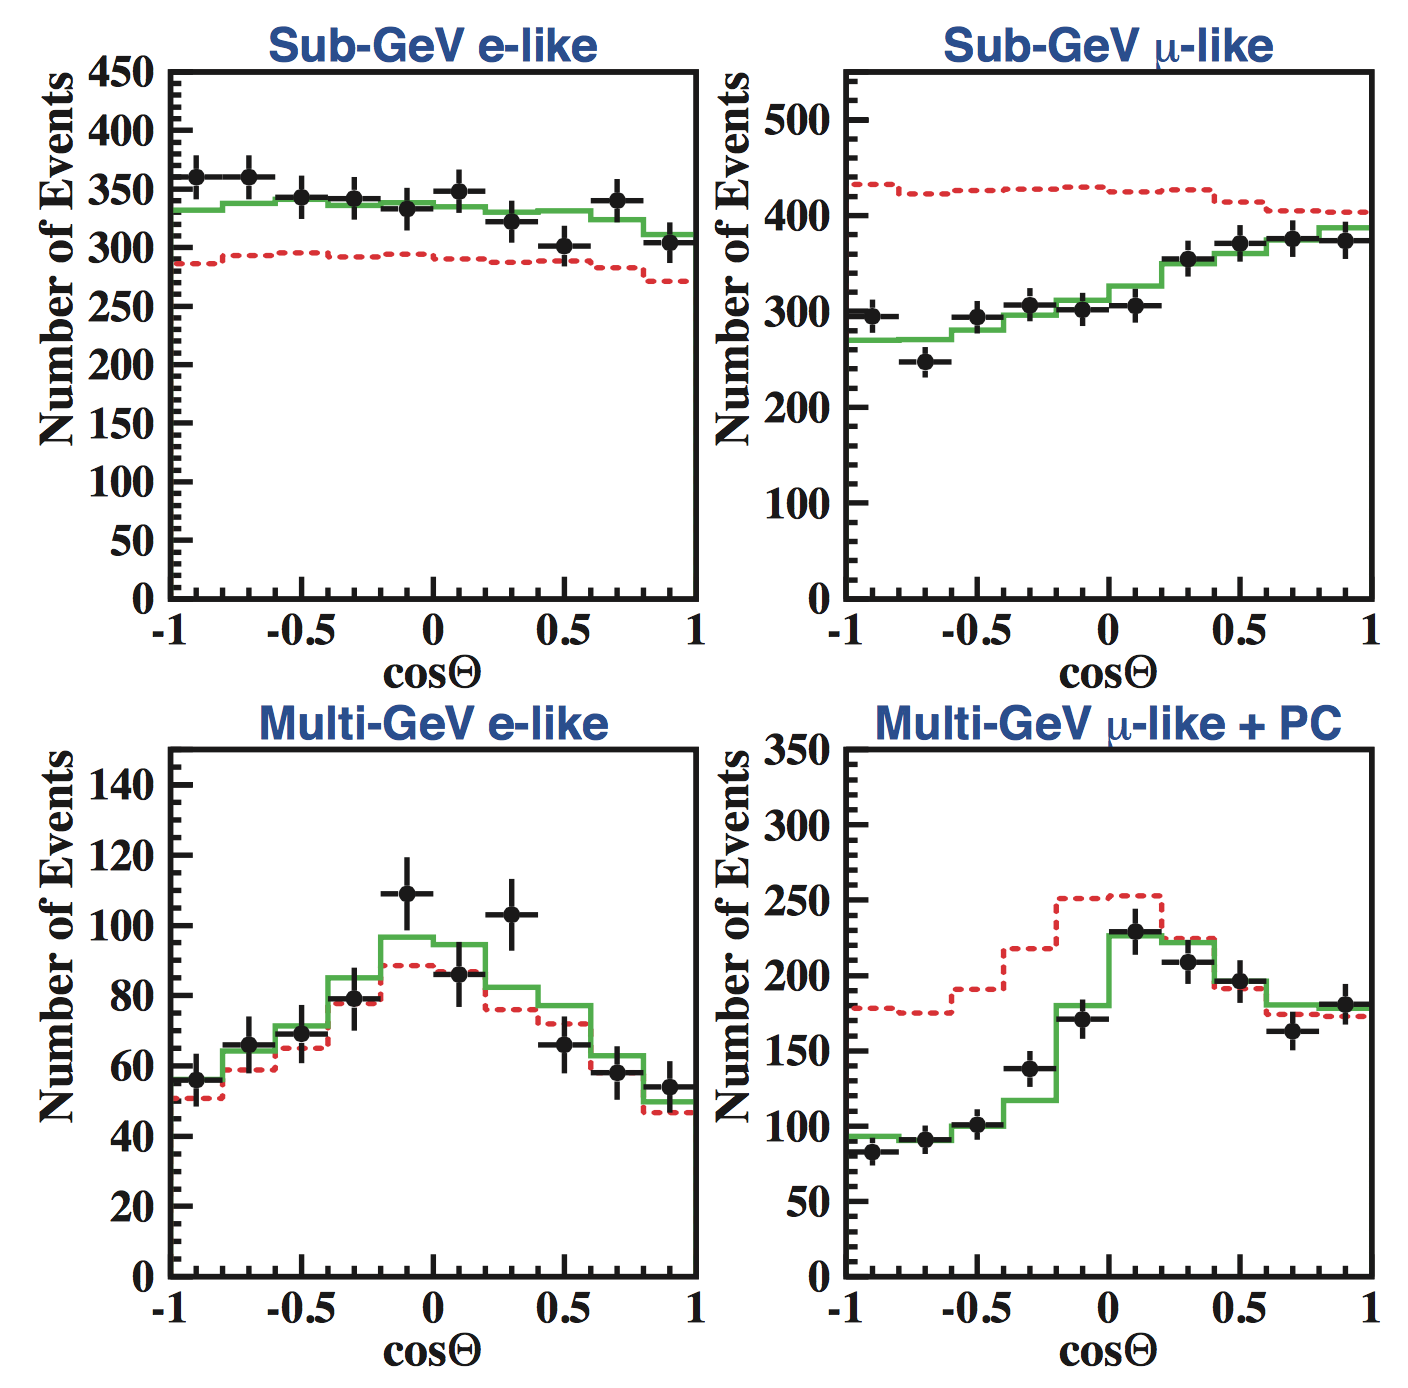
\includegraphics[width=1.0\textwidth]{./sk.png}
\end{figure}
\clearpage

Very intersting result.
Points are the observations, solid line is the prediction.
Notice a few think; For teh electrons everything works more or less OK, however for the muons it doesn work well at all.
You have an effect that says you dont understand what the muon \nus are doing and that effect dependson the energy and how far they are popogating.
\nus coming from above, \nus coming from below dont work well.  
Missing about half of them.

Very exciting result. B/c your sure the measurements are correct. 
Observable is robust. 
Implies that the \nus are doign someing. 
And whatever they are doing depends on the energy and the baseline (how much they have traveled)

Why is thsi important ? need a hypothesis for what is going on. 
Maybe the \nus are being absorbed ? 
\nus that go through the earth are gettins absorbed by the earth. 
Know Cant be true,  cross section would bave to be too high. 

What esle could be going on?
\nus decaying /changing flavour
Only looking for muon and electorn \nus, so if they were converting into $\tau$s, this could explain all this data.
Only massive particles know about time. 
What ever they are doing 
If \nus can tell time ==> \nus have mass. 
OR Lorentz invariance is wrong. 

So thats where we were. 
Bottom line \nus change flavour as a function of E and distance. 

\noindent\rule{\textwidth}{1pt}

\textbf{Mass-induced flavour oscillations.}

What happens if the \nus have mass ?

\be
\nu_1 \textrm{ with } m_1
\ee

\be
\nu_2 \textrm{ with } m_2
\ee

\be
\nu_3 \textrm{ with } m_3
\ee

If you raise the hypothesis that \nus have mass, then there are \nus states that you can label with different masses.

We also have \nue \numu and \nutau these are the interaction eigenstatss the \nus you produce when you have a weak interaction. 
The quesitno is then which one of these is the \nue \numu and \nutau ?


The answer is it doesnt have to be any of them, know for sureis that the \nue is a linear combination of \nus with a well-defined bass

\be
\nue = U_ei \nu_i
\ee

same for mus and taus. 

\be
\numu = U_mui \nu_i
\ee

\be
\nutau = U_taui \nu_i
\ee

also know that the \nue, \numu and \nutau or orthognal to one another (ie: they are different states) 

These Us can be organised into a unitary matrix. 

\be
\nualpha = U_{\alpha\ i} \nu_i
\ee

where, $\alpha = e, \mu, \tau$

i = 1,2,3

$U_{\alpha i}$ is Unitary mixing matrix
We will see, just by raising this hypothesis you can explain all the data.

\noindent\rule{\textwidth}{1pt}

Actually similar thing happens in the quark sector, we havent talked about this yet, but its true.

Have do identify who are the ``real particles''. 
Meaning what are the eigenstates of the free hamiltoninan.

In the quark section thats the 

u c t 
d s b

In the lepton sector we choose that to be 

e mu tau
nu1 nu2 nu3 

There is no such thing as an \nue, doesnt exist. 

but the weak interactions

$W \rightarrow t + b,s,b$ w/coupling $V_{CKM}$  $U_t,\alpha$

the same thing happens in the lepton sectior:


$W \rightarrow e + \nuone,\nutwo,\nuthree$ w/coupling $U_e,i$

physics is the same,  the consequesnces turn out to be very differnt.  
Main reaon is that the $\nu$ masses  are very small. 
Bc the masses are small (as well talk about in a second) you have a phenomina of $\nu$ oscillations.
Doesnt happen for quarks. 

\noindent\rule{\textwidth}{1pt}

OK lets set this up. 

What does it mean to be a particle with a well defined mass?
QM POV, eigen state of free particle hamiltoninaon. 

\be
\ket{\nuone} =  e^{-iE_1t} \ket{\nuone}
\ee

this is what ti means to be a $\nu$ with a well-defined mass.

Now What happens if you dont have one of these things, but a linear superposition of these. 

Lets say you have the \nue\ and to make life easy, lets pretend that we only have 2 \nus. 

Now \nue\ will be a linear combination of \nuone\ and \nutwo. 

\be
\ket{\nue} = \cos\theta \ket{\nuone} + \sin\theta \ket{\nutwo}
\ee

For completeness, can also write \numu, which is also a linear combination of \nuone\ and \nutwo, but it is a orthognal to \nue.

\be
\ket{\numu} = -\sin\theta \ket{\nuone} + \cos\theta \ket{\nutwo}
\ee


Some obvious things, we know $\cos\theta$ and $\sin\theta$ are some coefficients that we dont know, but we know the sum of squares is 1. 
(Thats why we write it like an angle) 

Can work this out from 
$\braket{\nue | \nue}  = 1$ and $\braket{\nue | \numu}  = 0$

thats why are allowed to paramaterize things in terms of an angle. 

How do these states evolve as a fucntion of time?

\be
\ket{\nue(t)} = \cos\theta e^{-iE_1t} \ket{\nuone} + \sin\theta e^{-iE_2t}\ket{\nutwo}
\ee

this is the heart of what $\nu$ oscillations are all about. 
Because these phaces are different, what you get is no longer proportinal to the \nue\ state.
Or in fancier words, \nue\ is not an eigenstate of the free hamiltonian.

NOw this is very very simple physics. 
Literally a 2 level system that you learned in undergraduate QM.


Rember everything is going to be relativistic. 
\nus are going to be propogating plane waves. 

Relativistic version 

\be
\ket{\nue(\vec{x},t)} = \cos\theta e^{-ip_1^\mu x_\mu} \ket{\nuone} + \sin\theta e^{-ip_2^\mu x_\mu}\ket{\nutwo}
\ee
where x is the $(t,\vec{x})$ four vector. 

\textbf{Ultra relativistic approx. }

\be
t \sim L 
\ee

Phase factors very close to being zero, depend on difference between energy and momentum $(E_1 - p_1)$


Now let me calculate this differnce in the following way,
\be
(E_1 - p_1)(E_1 + p_1) = m_1^2  \Rightarrow  (E_1 - p_1) = \frac{m_1^2}{2E} 
\ee
in the ultra relativistic approx $E \sim P$


\be
\ket{\nue(L)} = \cos\theta e^{-i \frac{m_1^2}{2E} L} \ket{\nuone} + \sin\theta e^{-i \frac{m_2^2}{2E} L} \ket{\nutwo}
\ee

OK, now lets calculate something...


Lets calculate the probablity that this obect here, when it hits something produces an electron. 

Which is just given by 

\be
\braket{\nue | \nue(L) } = \cos^2 \theta e^{-i \frac{m_1^2}{2E} L} + \sin^2\theta e^{-i \frac{m_2^2}{2E} L} 
\ee

Amplitude for having an \nue\ be born somewhere, propagate some distance L and then be detected as an \nue.

So the proabablity is this thing squared

\begin{eqnarray*}
\left|\braket{\nue | \nue(L) }\right|^2 &=& \left|\cos^2 \theta e^{-i \frac{m_1^2}{2E} L} + \sin^2\theta e^{-i \frac{m_2^2}{2E} L} \right|^2\\
       &=& \left|\cos^2 \theta+ \sin^2\theta e^{-i \frac{m_2^2 - m_1^2}{2E} L} \right|^2\\
       &=& \cos^4 \theta+ \sin^4\theta  + \cos^2\theta \sin^2 \theta 2 \cos \left( \frac{\Delta m^2 L}{2E} \right)
\end{eqnarray*}
where $\Delta m^2 = m_2^2 - m_1^2$


Can simply this...

\begin{eqnarray*}
 &=& \left( \cos^2 \theta + \sin^2 \theta \right)^2  - 2 \cos^2 \theta \sin^2 \theta  + 2 \cos^2 \theta \sin^2 \theta \cos \left( \frac{\Delta m^2 L}{2E} \right) \\
 &=& 1 - 2 \cos^2 \theta \sin^2 \theta \left( 1  - \cos \left( \frac{\Delta m^2 L}{2E} \right) \right)
\end{eqnarray*}


Now use a trig ID for $1-\cos\theta$...

\begin{eqnarray*}
 &=& 1 - 4 \sin^2 \theta \cos^2 \theta \sin^2 \left( \frac{\Delta m^2 L}{2E} \right)\\
 &=& 1 -  \sin^2 2\theta \sin^2 \left( \frac{\Delta m^2 L}{2E} \right)
\end{eqnarray*}

So what we learn at the end of the day is, if your born as \nue and you propogate a certian distance L, and you're detectred as an \nue, the probablity is given by,

\be 
P_ee(L) = 1 - \sin^2 2\theta \sin^2 \left( \frac{\Delta m^2 L}{2E} \right)
\ee 
Possible to be born as \nue and detected as \nue with less than 100\% probability.

}
\end{document}


